%--------------------------------------------------
\subsection{Prototipo 4: Integración de sistema de recomendación basado en filtrado colaborativo segunda versión}
Dentro del análisis para el desarrollo de este prototipo se incorporan los siguientes requerimientos funcionales: \\
\begin{itemize}
	\item \hyperlink{RFSGPyPDR}{RFGPPR3 Generar módulo de recomendaciones basado el filtrado colaborativo.}
	\item \hyperlink{RFSGPyPDR}{RFGPPR22 Obtener recomendaciones globales}
	\item \hyperlink{RFSGPyPDR}{RFGPPR23 Obtener recomendaciones por departamento.}
\end{itemize}

definidos previamente en el capítulo del ``Bosquejo general de la aplicación''  con el título de ``Requerimientos funcionales del Sistema de Gestión, Procesamiento y Proveedor de Datos Retail''. \\ \par

\title{\textbf{Simbología necesaria:}
\\W := Matriz de pesos de los usuarios.
\\X := Matriz de pesos de productos.
\\p := valor de la predicción.
\\$ W^{(usuario)}$ := Vector de pesos de un usuario.
\\$ X^{(producto)}$ := Vector de pesos de un producto.
\\$ y^{(i,j)}$ := Calificación para el producto i hecha por el usuario j. 
\\$ r(i,j) = 1$ := Producto i calificado por usuario j.\\
%--------------------------------------------------
\subsubsection{Análisis}
Durante esta sección se explicarán algunas mejoras aplicadas al algoritmo de Filtrado Colaborativo.
\\\\\textbf{Función de error}\\
La función de error sigue siendo el \textbf{Error cuadrático medio} pero como se puede observar en la ecuación \ref{equation:J} existen dos sumatorias que corresponden a una técnica llamada Regularización, esta técnica nos permite poner una cota superior para los valores de los vectores X y W con el objetivo de evitar el famoso sobreentrenamiento.
\begin{equ}[!ht]
  \begin{equation}
  \begin{array}{c}
	J = \frac{1}{num.productos} \sum_{i}^{num.productos} \sum_{j}^{num.usuarios} ({W^{(j)}}^{T}X^{(i)} - y^{(i,j)})^2  \\
	+ \frac{\lambda}{num.productos} \sum_{k=1}^{num.productos} {X^{(k)}}^2 
	+ \frac{\lambda}{num.usuarios} \sum_{k=1}^{num.usuarios} {W^{(k)}}^2 
  \end{array}
  \end{equation}
 \caption{Definición matemática de la función de error.}
  \label{equation:J}
\end{equ}
\FloatBarrier
%%%%%%%%%%%%%%%%%%%%%%%%%%%%%
\title{\textbf{\\Mean Normalization}
\\\textbf{Introducción al problema}
\FloatBarrier
\begin{figure}[htbp!]
		\centering
			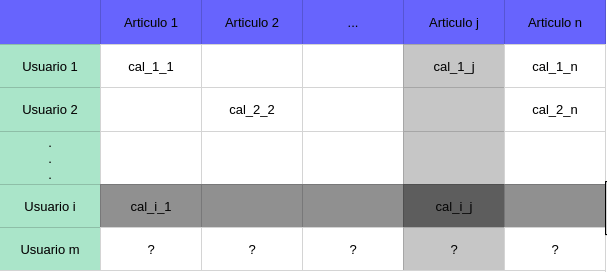
\includegraphics[width=0.7 \textwidth]{imagenes/sistemarec/matrizusuarionuevo}
		\caption{Matriz Artículo-Usuario con usuario nuevo.}
		\label{usuarionuevomatriz}
\end{figure}
\FloatBarrier

En la figura \ref{usuarionuevomatriz} se puede observar una Matriz Artícuo-Usuario con un usuario nuevo sin compras ni calificaciones. Dentro de esta matriz se genera un problema: éste surge al realizar las predicciones, ya que, el vector de pesos (W) contiene unicamente ceros y al realizar la predicción de algún producto esta es cero para cualquier X.

\textbf{Solución} \linebreak
Mean normalization es una técnica que consiste en obtener la media de las calificaciones dada a algún productos por los usuarios que han adquirido dicho producto. En términos matemáticos significa lo siguiente: 
\FloatBarrier

\begin{equ}[!ht]
  \begin{equation}
         \frac{\sum_{i: r(i,producto) = 1}^{num_usuarios} y^{producto,i}}{\sum_{i: r(i,producto) = 1}^{num_usuarios} 1} = \mu_{producto}
  \end{equation}
 \caption{Definición matemática de Mean normalization.}
  \label{equation:hiperplano}
\end{equ}
\FloatBarrier

Una vez obtenida la calificación media de cada producto se tiene que sustraer dicha media de la calificación que le había asignado el usuario.
\\Finalmente, tomando en cuenta la calificación media del producto las predicciones cambian a la siguiente manera:
\begin{equ}[!ht]
  \begin{equation}
        \ p = W^{T}X^{producto} + \mu_{producto} 
  \end{equation}
 \caption{Definición matemática de predicción con Mean normalization.}
  \label{equation:prediccion}
\end{equ}
\FloatBarrier
\title{\textbf{\\Mejoras en tiempos de respuesta}
\\En el prototipo 3 llamado \textbf{Integración de sistema de recomendación basado en filtrado colaborativo primera versión} se ejecutaba el algoritmo cada vez que algún usuario cliente o usuario vendedor realizaban una petición, el tiempo de respuesta aproximado para recomendaciones globales era de 30 minutos y el tiempo aproximado para recomendaciones por departamento era de 5 segundos.\\\\
\textbf{¿Cómo se mejoró el tiempo de respuesta?}
\\Se escribió un script en python que debe ser ejecutado cada cierto para tener las  recomendaciones globales \textbf{precargadas} en archivos json con que tienen como nombre el identificador único de cada cliente. De igual manera, cada vez que se ejecuta dicho script en el repositorio de datos son almacenados los valores optimizados de los vectores X y W, de esta manera cada vez que se hace una petición de recomendaciones por departamentos simplemente se calculan las predicciones con la ecuación \ref{equation:prediccion}. \\\\
\textbf{¿Qué pasa cuando un cliente nuevo entra al sistema y no tiene aún su archivo de recomendaciones globales precargado?}
\\Al no tener un archivo con sus recomendaciones precargadas significa que el script de python que lo genera aún no ha sido ejecutado y por ende su vector de W está completamente en ceros. La solución al problema es simplemente aplicar la ecuación \ref{equation:prediccion} por cuestiones de tiempos de respuesta, se decidió simplemente hacer una consulta al repositorio de datos buscando los cien productos productos con mayor calificación media (esto nos proporciona el mismo resultado que la ecuación \ref{equation:prediccion}); de esta manera a un usuario nuevo se le hacen recomendaciones de los productos que más le han gustado a todos los clientes.

%--------------------------------------------------
\subsubsection{Diseño}

%%%%%%%%%%%%%%%%%%%%%%%%%%%%%%%%%%%%%%%%%%%%%%%%%%%%%%%%%%%%%%%
\title{\textbf{RFGPPR22 Obtener recomendaciones globales}
\begin{itemize}
\item Ruta: /client/get-global-recom/{id\_usuario}
\begin{itemize}
\item Método: GET
\item Tipo de parámetro: ruta
\item Opciones [id\_usuario, int]
\item Respuesta exitosa:
\begin{lstlisting}[language=json,firstnumber=1]
{	"products": [{
		"id_producto" : integer,
		"producto": "string",
		"precio_venta" : "string",
		"stock" : integer,
		"departamento" : "string",
		"tienda" : "string",
		"categoria" : "string",
		"marca" : "string",
		"promocion" : "string",
		"imagen": "string"
		"score" : float
},
{...},
{...},
...]}
\end{lstlisting}

\item Respuesta erronea:
\begin{lstlisting}[language=json,firstnumber=1]
{
    "message": "string",
}
\end{lstlisting}
\end{itemize}
\end{itemize}

%%%%%%%%%%%%%%%%%%%%%%%%%%%%%%%%%%%%%%%%%%%%%%%%%%%%%%%%%%%%%%%%%%
\title{\textbf{RFGPPR23 Obtener recomendaciones por departamento.}
\begin{itemize}
\item Ruta: /client/recommendations/department/(id\_usuario)/{id\_departamento}
\begin{itemize}
\item Método: GET
\item Tipo de parámetro: ruta
\item Opciones [id\_usuario, int], [id\_departamento, int]
\item Respuesta exitosa:
\begin{lstlisting}[language=json,firstnumber=1]
{	"products": [{
		"id_producto" : integer,
		"producto": "string",
		"precio_venta" : "string",
		"stock" : integer,
		"departamento" : "string",
		"tienda" : "string",
		"categoria" : "string",
		"marca" : "string",
		"promocion" : "string",
		"imagen": "string"
		"score" : float
},
{...},
{...},
...]}
\end{lstlisting}

\item Respuesta erronea:
\begin{lstlisting}[language=json,firstnumber=1]
{
    "message": "string",
}
\end{lstlisting}
\end{itemize}
\end{itemize}

\subsection{Pruebas}
\textit{Las pruebas del sistema fueron hechas sobre una laptop Lenovo Thinkpad T460 con las siguientes carácteristicas:\\}
\begin{itemize}
\item Procesador Intel® Core™ i5-5300U (3M Cache, hasta 2,90 GHz).
\item 8 GB RAM.
\item 240 GB Solid State Drive ROM.
\item Sistema Operativo Fedora 27.
\end{itemize}
\textit{Nota: Durante estas pruebas se agregó la regularización}

%%%%%%%%%%%%%%%%%%%%% PRUEBA 1
\title{\textbf{Prueba 1.}}

\begin{itemize}
\item Número de clientes:184
\item Número de productos: 10001
\item Número de compras: 144192
\item Número de iteraciones: 30
\item Número de parámetros: 13
\item Tasa de aprendizaje: 0.01
\item Regularización: 0.01
\end{itemize}
\newpage
\textbf{Prueba con validación: 70\% entrenamiento 30\% validación}

\FloatBarrier
\begin{figure}[htbp!]
		\centering
			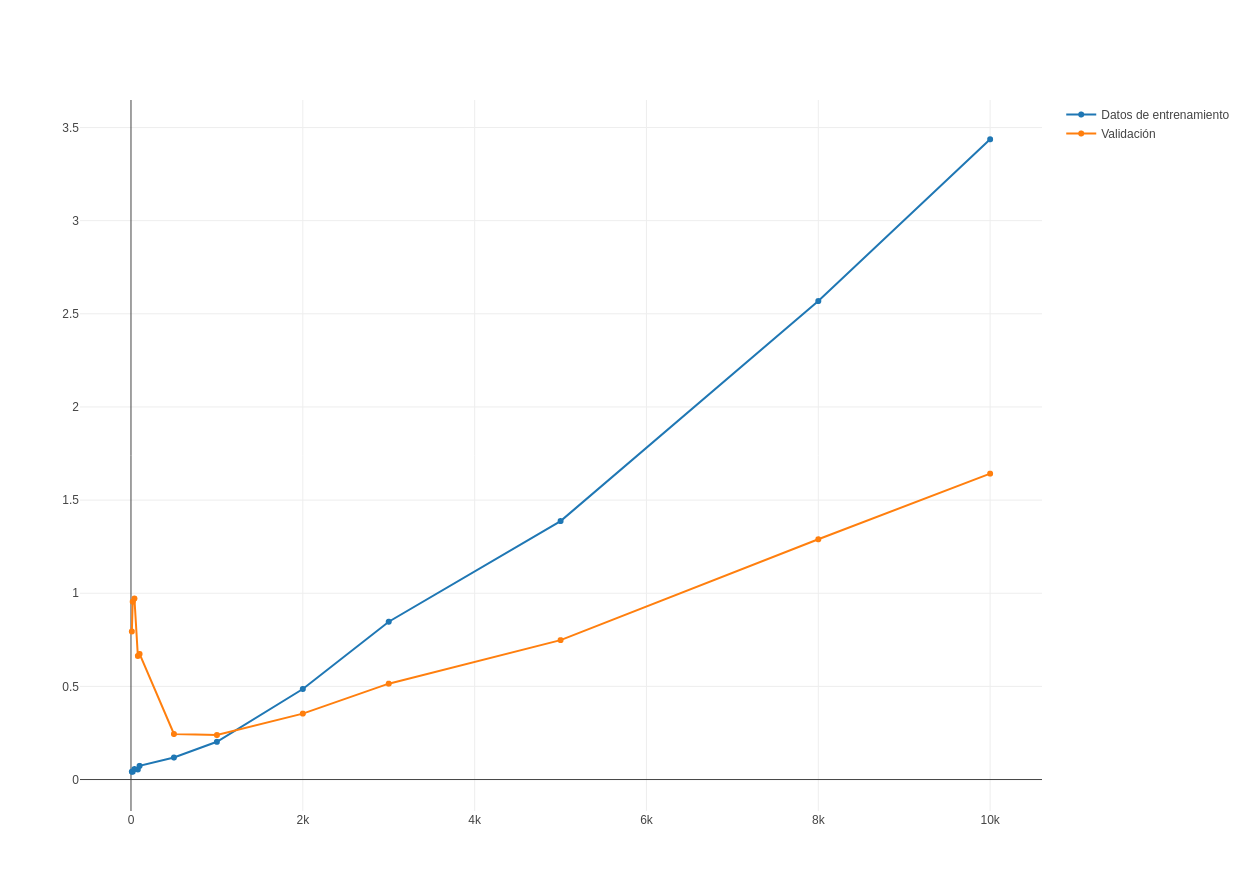
\includegraphics[width=1 \textwidth]{imagenes/pruebassistemarecom/30_01_13}
		\caption{Prueba 1 con validación.}
		\label{gradiente_desc}
\end{figure}
\FloatBarrier
\newpage
\textbf{Prueba de J respecto al número de iteraciones}

\FloatBarrier
\begin{figure}[htbp!]
		\centering
			
\includegraphics[width=1 \textwidth]{imagenes/pruebassistemarecom/2_1}
		\caption{Prueba 1 con regularización: J respecto al número de iteraciones.}
		\label{gradiente_desc}
\end{figure}
\FloatBarrier
%%%%%%%%%%%%%%%%%%%%% PRUEBA 2
\title{\textbf{Prueba 2.}}

\begin{itemize}
\item Número de clientes:184
\item Número de productos: 10001
\item Número de compras: 144192
\item Número de iteraciones: 100
\item Número de parámetros: 13
\item Tasa de aprendizaje: 0.01
\item Regularización: 0.000001
\end{itemize}
\newpage
\textbf{Prueba con validación: 70\% entrenamiento 30\% validación}
\FloatBarrier
\begin{figure}[htbp!]
		\centering
			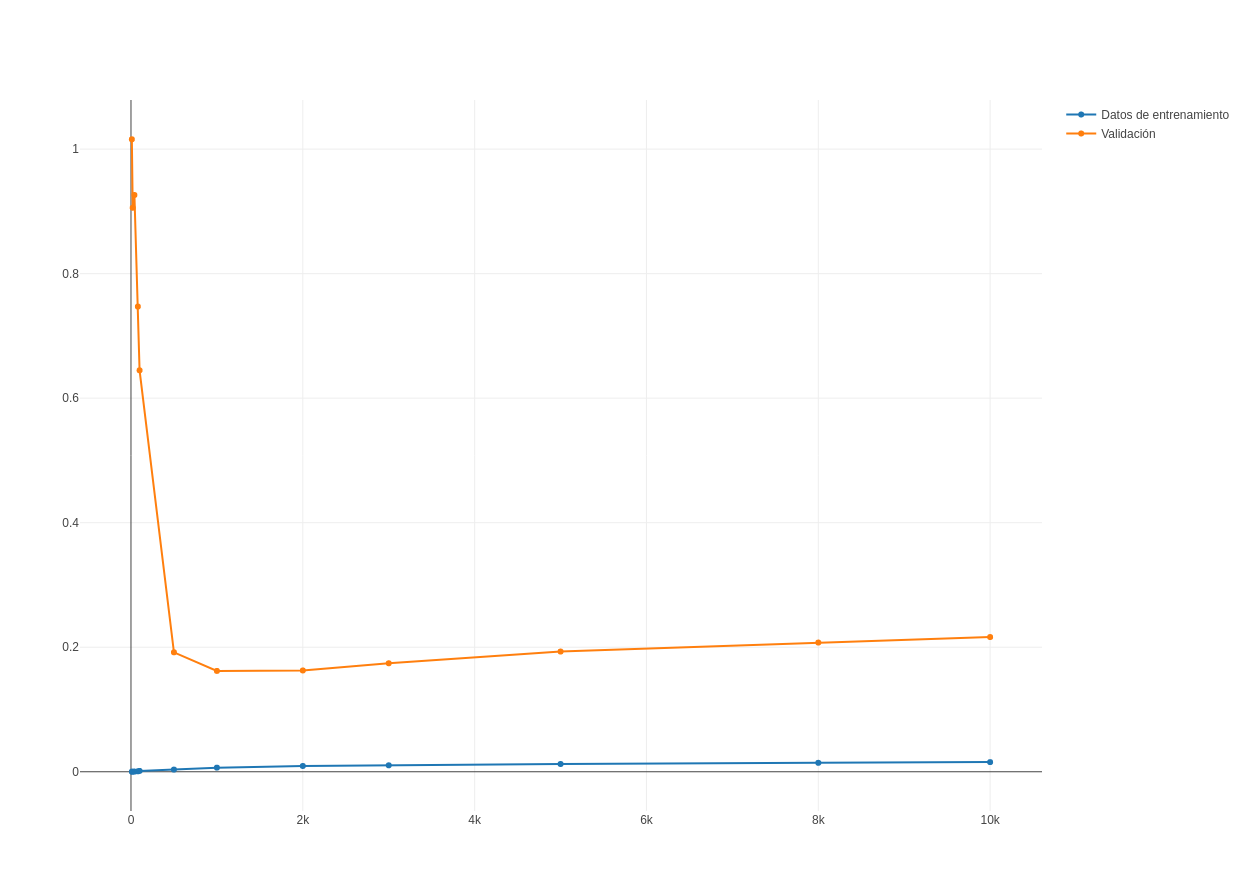
\includegraphics[width=1 \textwidth]{imagenes/pruebassistemarecom/100_000001_13}
		\caption{Prueba 2 con validación.}
		\label{gradiente_desc}
\end{figure}
\FloatBarrier
\newpage
\textbf{Prueba de J respecto al número de iteraciones}

\FloatBarrier
\begin{figure}[htbp!]
		\centering
			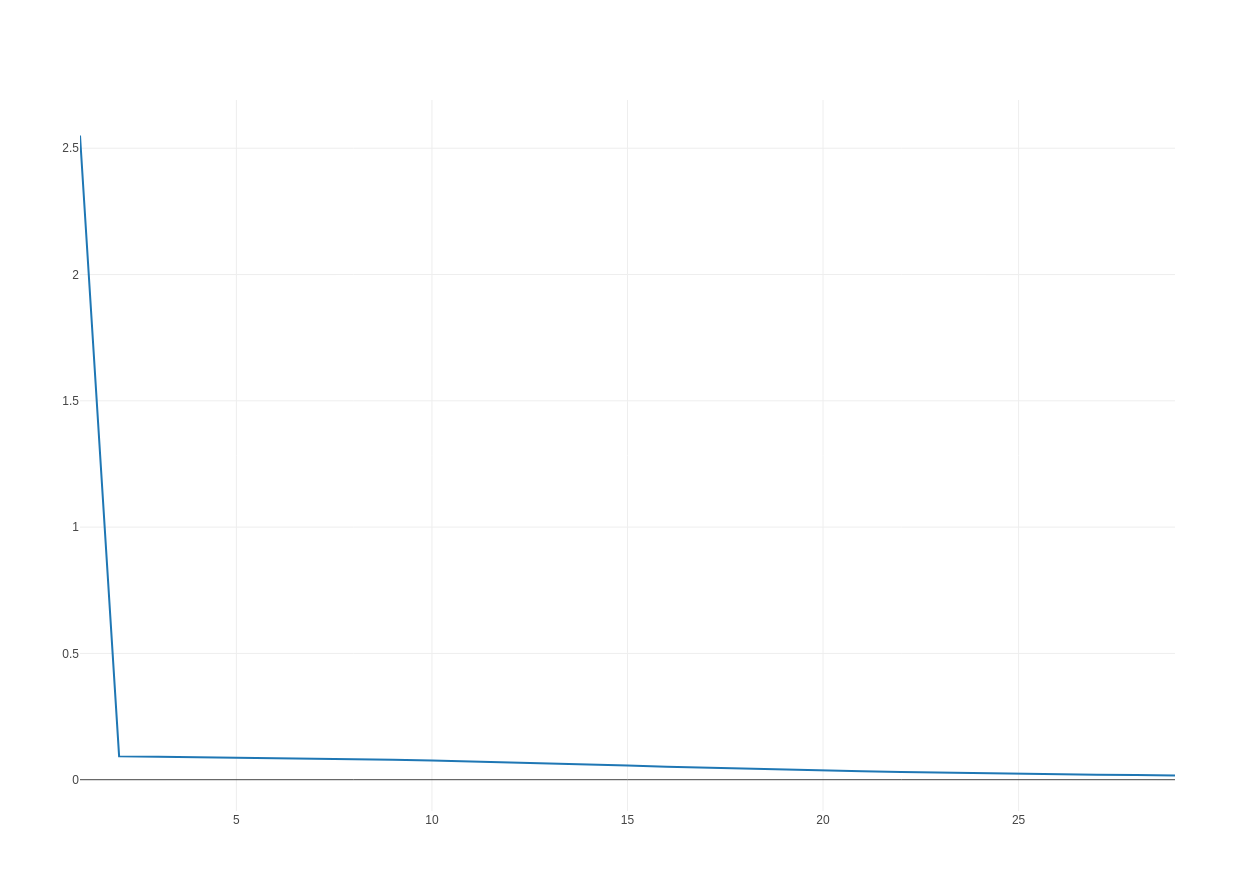
\includegraphics[width=1 \textwidth]{imagenes/pruebassistemarecom/1_j}
		\caption{Prueba 2 con regularización: J respecto al número de iteraciones.}
		\label{gradiente_desc}
\end{figure}
\FloatBarrier

%%%%%%%%%%%%%%%%%%%%% PRUEBA 3
\title{\textbf{Prueba 3.}}

\begin{itemize}
\item Número de clientes:184
\item Número de productos: 10001
\item Número de compras: 144192
\item Número de iteraciones: 100
\item Número de parámetros: 15
\item Tasa de aprendizaje: 0.01
\item Regularización: 0.000001
\end{itemize}
\newpage
\textbf{Prueba con validación: 70\% entrenamiento 30\% validación}

\FloatBarrier
\begin{figure}[htbp!]
		\centering
			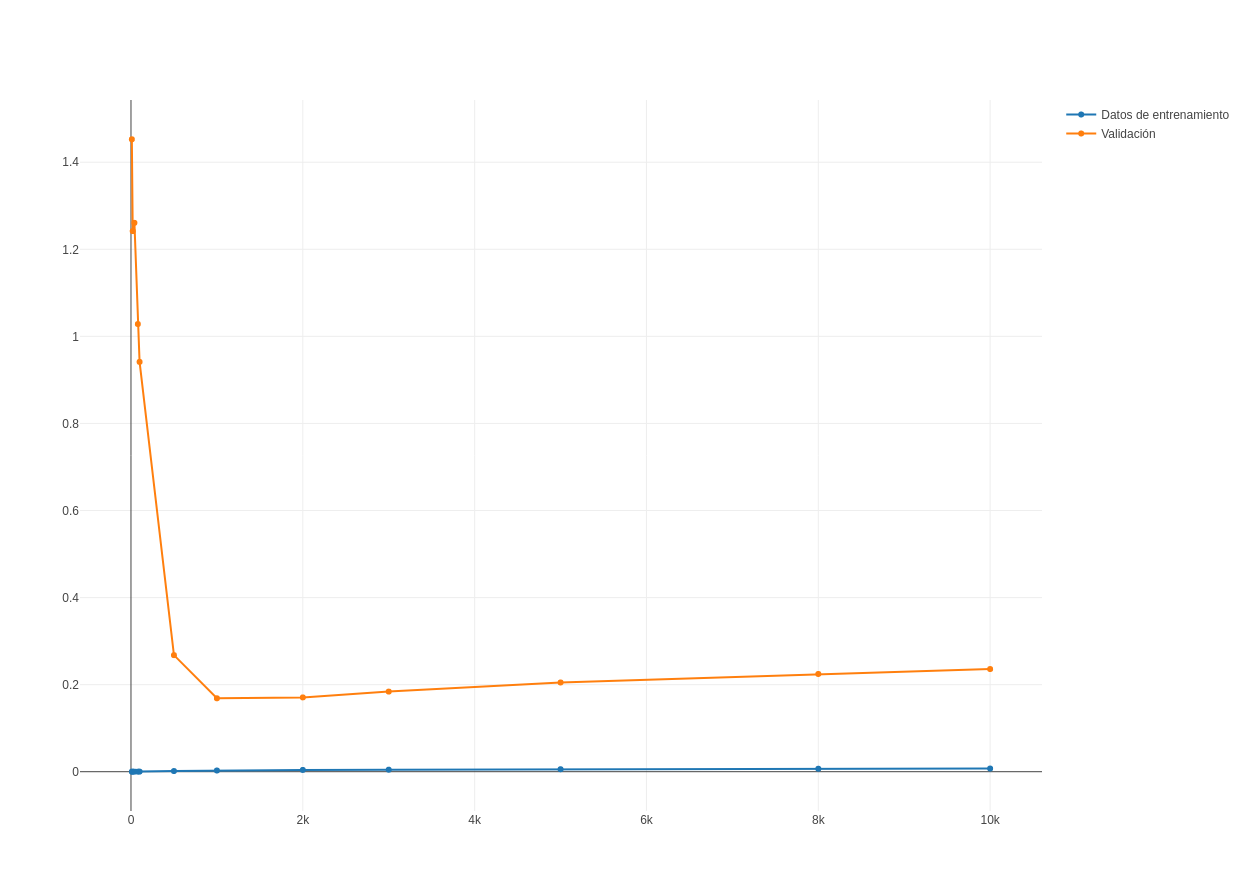
\includegraphics[width=1 \textwidth]{imagenes/pruebassistemarecom/100_000001_15}
		\caption{Prueba 3 con validación.}
		\label{gradiente_desc}
\end{figure}
\FloatBarrier
\newpage
\textbf{Prueba de J respecto al número de iteraciones}

\FloatBarrier
\begin{figure}[htbp!]
		\centering
			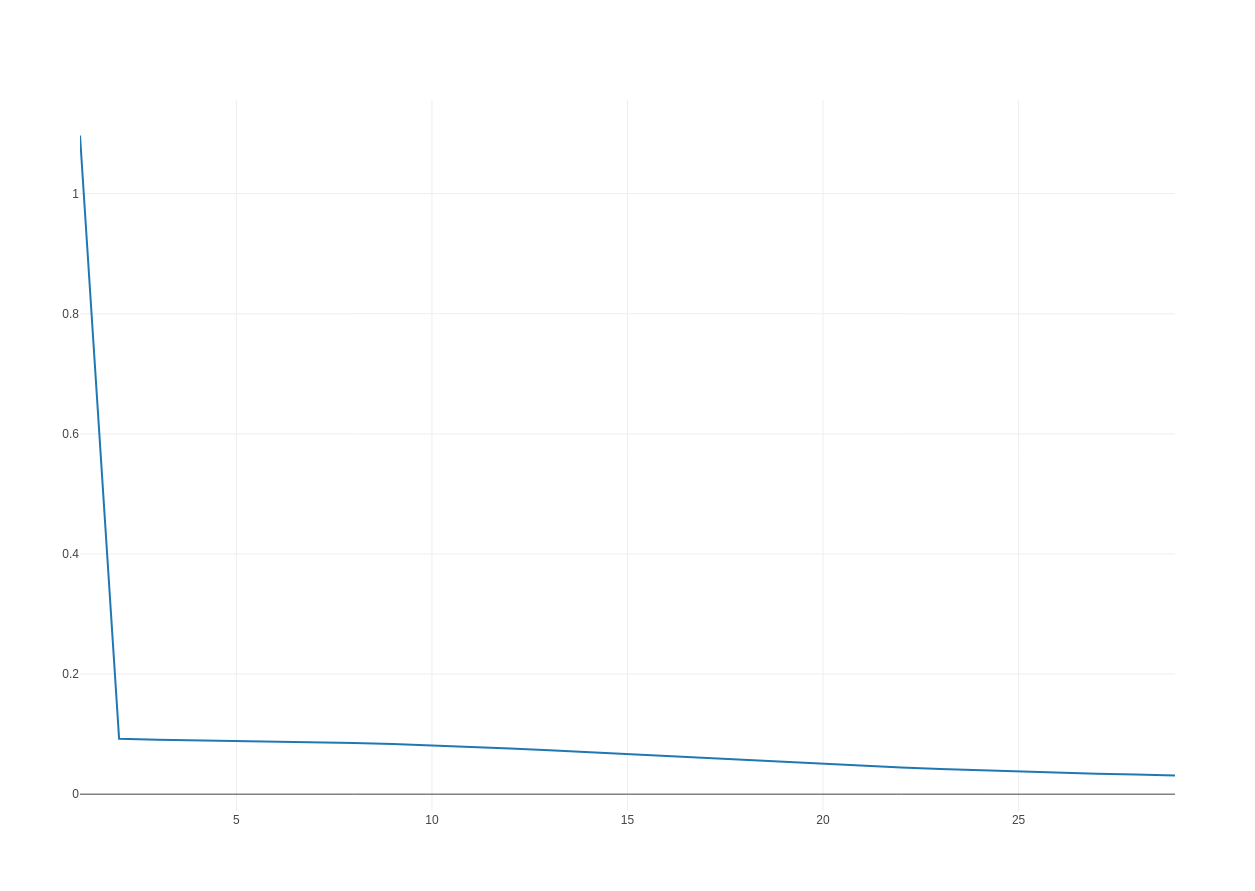
\includegraphics[width=1 \textwidth]{imagenes/pruebassistemarecom/2_3}
		\caption{Prueba 3 con regularización: J respecto al número de iteraciones.}
		\label{gradiente_desc}
\end{figure}
\FloatBarrier

%%%%%%%%%%%%%%%%%%%%% PRUEBA 4
\title{\textbf{Prueba 4.}}

\begin{itemize}
\item Número de clientes:184
\item Número de productos: 10001
\item Número de compras: 144192
\item Número de iteraciones: 5
\item Número de parámetros: 13
\item Tasa de aprendizaje: 0.01
\item Regularización: 0.0000000005
\end{itemize}
\newpage
\textbf{Prueba con validación: 70\% entrenamiento 30\% validación}

\FloatBarrier
\begin{figure}[htbp!]
		\centering
			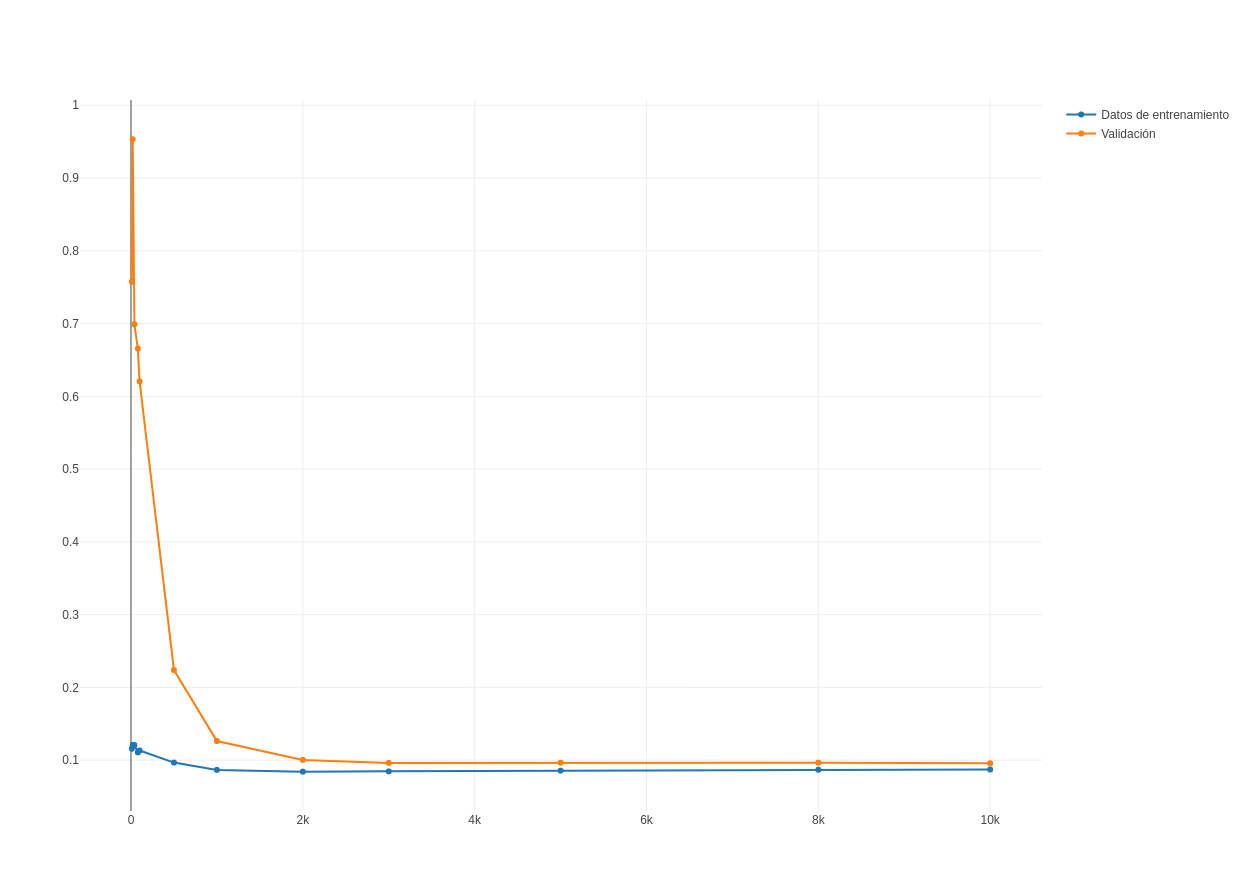
\includegraphics[width=1 \textwidth]{imagenes/pruebassistemarecom/5_0000000005_13}
		\caption{Prueba 3 con validación.}
		\label{pruebabien}
\end{figure}
\FloatBarrier
\newpage
\textbf{Prueba de J respecto al número de iteraciones}

\FloatBarrier
\begin{figure}[htbp!]
		\centering
			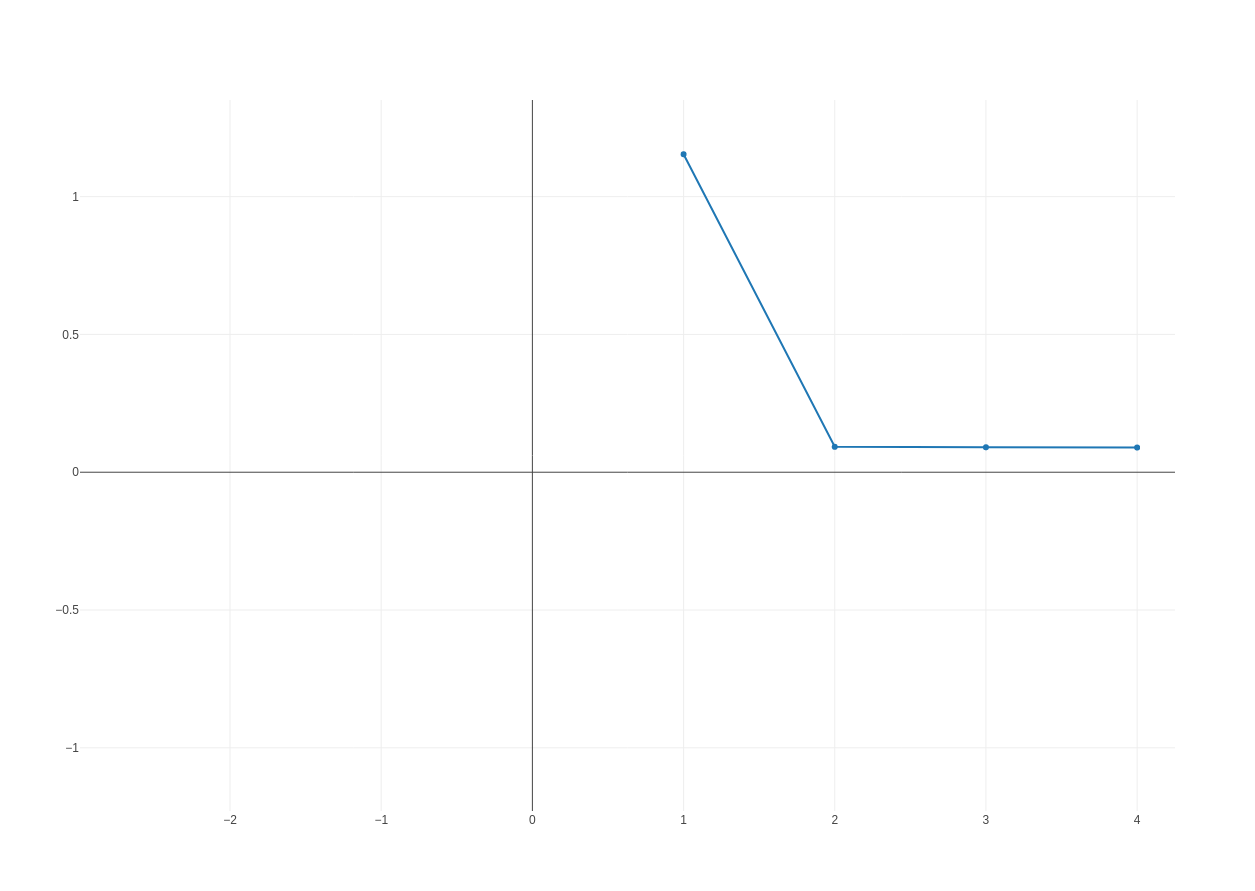
\includegraphics[width=1 \textwidth]{imagenes/pruebassistemarecom/2_4}
		\caption{Prueba 3 con regularización: J respecto al número de iteraciones.}
		\label{gradiente_desc}
\end{figure}
\FloatBarrier

%%%%%%%%%%%%%%%%%%%%% PRUEBA 5
\title{\textbf{Prueba 5.}}

\begin{itemize}
\item Número de clientes:184
\item Número de productos: 10001
\item Número de compras: 144192
\item Número de iteraciones: 10
\item Número de parámetros: 13
\item Tasa de aprendizaje: 0.01
\item Regularización: 0.0000000005
\end{itemize}
\newpage
\textbf{Prueba con validación: 70\% entrenamiento 30\% validación}

\FloatBarrier
\begin{figure}[htbp!]
		\centering
			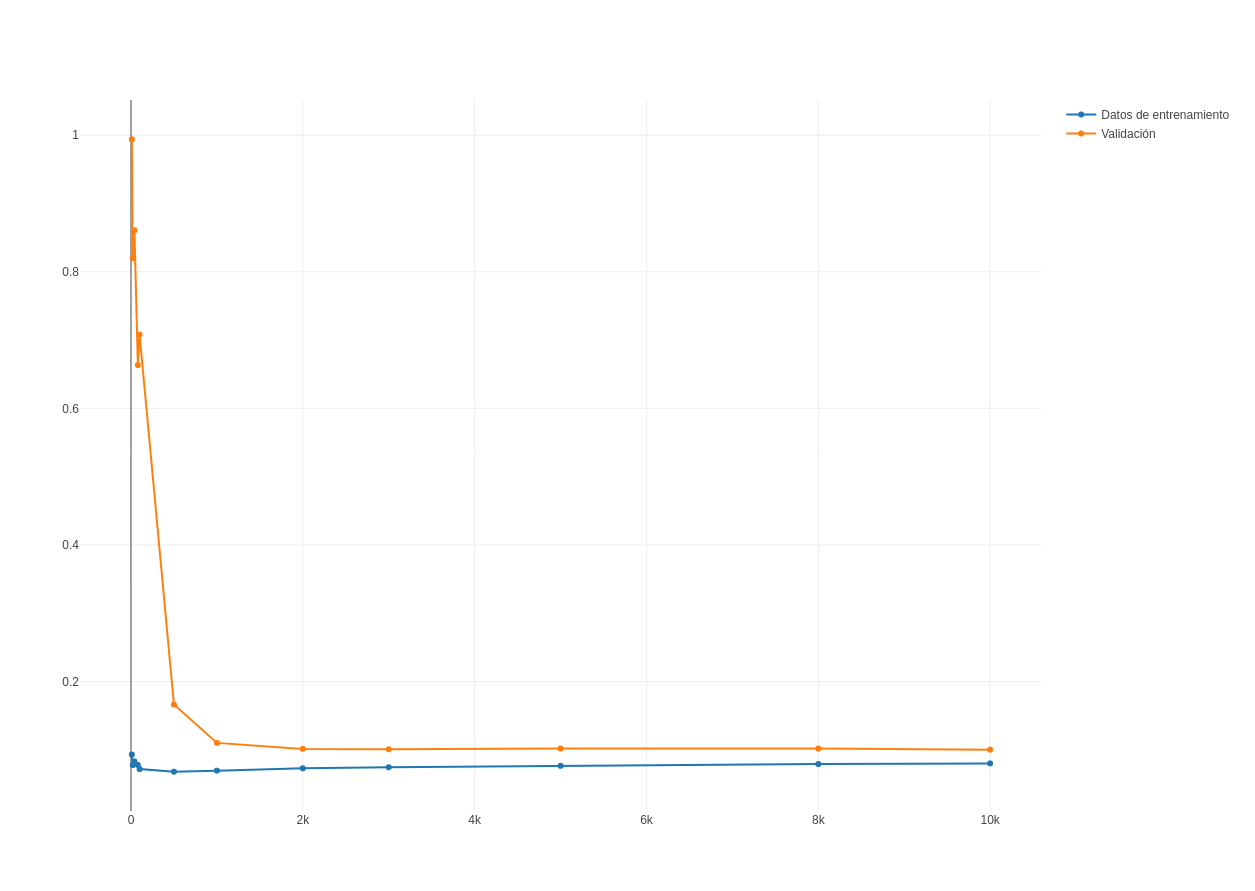
\includegraphics[width=1 \textwidth]{imagenes/pruebassistemarecom/10_0000000005_13}
		\caption{Prueba 3 con validación.}
		\label{gradiente_desc}
\end{figure}
\FloatBarrier
\newpage
\textbf{Prueba de J respecto al número de iteraciones}

\FloatBarrier
\begin{figure}[htbp!]
		\centering
			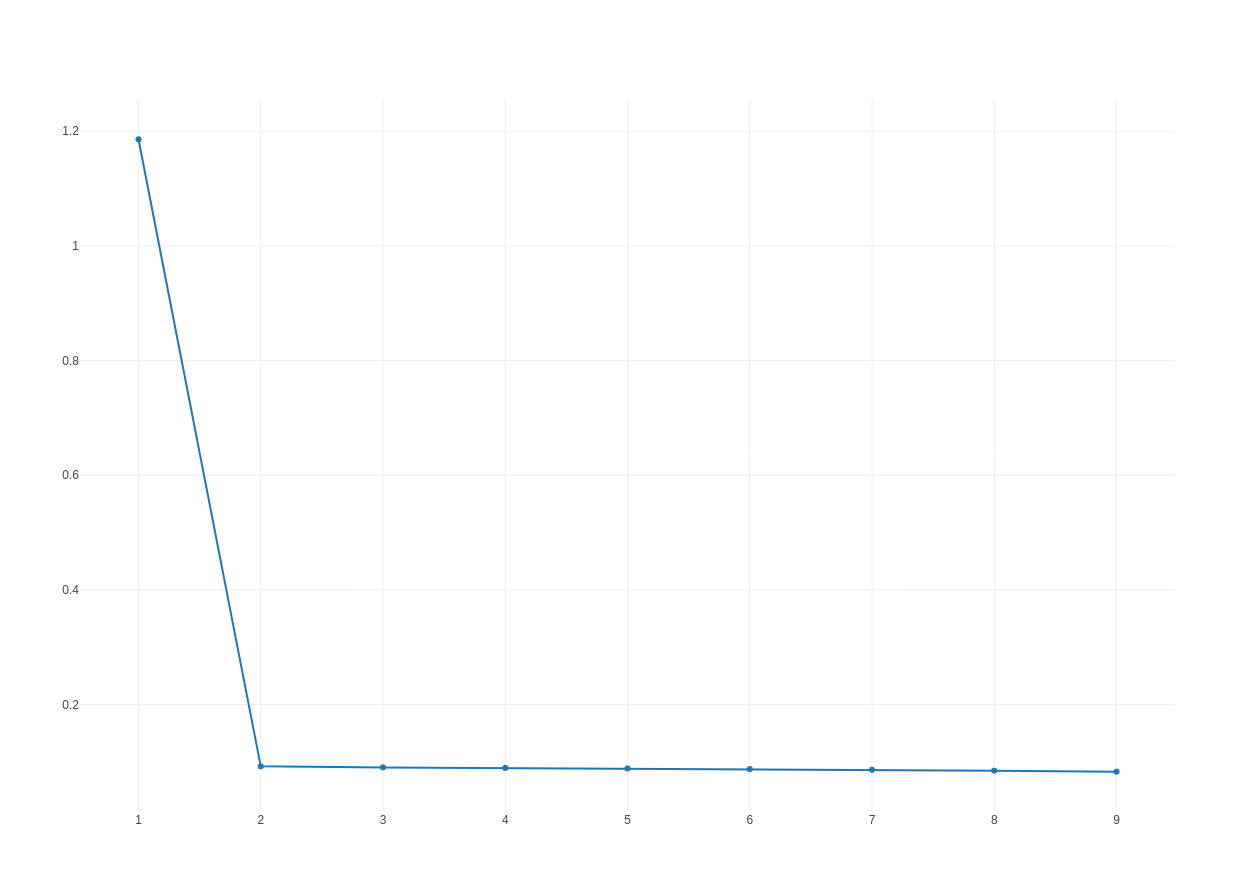
\includegraphics[width=1 \textwidth]{imagenes/pruebassistemarecom/2_5}
		\caption{Prueba 3 con regularización: J respecto al número de iteraciones.}
		\label{gradiente_desc}
\end{figure}
\FloatBarrier


\subsubsection{Conclusiones}
De acuerdo con las pruebas realizadas se decidió que la prueba número tres con regularización es la óptima, ya que, como se muestra en la gráfica \ref{pruebabien} los datos de entrenamiento y validación tienen una convergencia muy cercana aproximadamente en 0.1. Por otro lado, dicha gráfica nos corrobora que no existe el sobreentrenamiento en nuestro modelo.  
